% move all configuration stuff into one file so we can focus on the content
\documentclass[aspectratio=169,hyperref={pdfpagelabels=false,colorlinks=true,linkcolor=white,urlcolor=blue},t]{beamer}

%%%%%%%%%%%%%%%%%%%%%%%%%%%%%%%%%%%%%%%%%%%%%%%%%%%%%%%%%%%%%%%%%%%%%%%%%%%%%%%%%%
%%%%%%%%%%%%%%%%%%%%%%%%%%%%%%%%%%%%%%%%%%%%%%%%%%%%%%%%%%%%%%%%%%%%%%%%%%%%%%%%%%
% packages
\usepackage{pict2e}
\usepackage{epic}
\usepackage{amsmath,amsfonts,amssymb}
\usepackage{units}
\usepackage{fancybox}
\usepackage[absolute,overlay]{textpos} 
\usepackage{media9} % avi2flv: "C:\Program Files\ffmpeg\bin\ffmpeg.exe" -i TuneFreqFilterbank.avi -b 600k -s 441x324 -r 15 -acodec copy TuneFreqFilterbank.flv
\usepackage{animate}
\usepackage{gensymb}
\usepackage{multirow}
\usepackage{silence}
\usepackage[backend=bibtex,style=ieee]{biblatex}
\AtEveryCitekey{\iffootnote{\tiny}{}}
\addbibresource{references}

%%%%%%%%%%%%%%%%%%%%%%%%%%%%%%%%%%%%%%%%%%%%%%%%%%%%%%%%%%%%%%%%%%%%%%%%%%%%%%%%%%
%%%%%%%%%%%%%%%%%%%%%%%%%%%%%%%%%%%%%%%%%%%%%%%%%%%%%%%%%%%%%%%%%%%%%%%%%%%%%%%%%%
% relative paths
\graphicspath{{graph/}}


%%%%%%%%%%%%%%%%%%%%%%%%%%%%%%%%%%%%%%%%%%%%%%%%%%%%%%%%%%%%%%%%%%%%%%%%%%%%%%%%%%
%%%%%%%%%%%%%%%%%%%%%%%%%%%%%%%%%%%%%%%%%%%%%%%%%%%%%%%%%%%%%%%%%%%%%%%%%%%%%%%%%%
% units
\setlength{\unitlength}{1mm}

%%%%%%%%%%%%%%%%%%%%%%%%%%%%%%%%%%%%%%%%%%%%%%%%%%%%%%%%%%%%%%%%%%%%%%%%%%%%%%%%%%
%%%%%%%%%%%%%%%%%%%%%%%%%%%%%%%%%%%%%%%%%%%%%%%%%%%%%%%%%%%%%%%%%%%%%%%%%%%%%%%%%%
% theme & layout
\usetheme{Frankfurt}
\beamertemplatenavigationsymbolsempty
%\setbeamertemplate{frametitle}[smoothbars theme]
\setbeamertemplate{frametitle}
{
    \begin{beamercolorbox}[ht=1.8em,wd=\paperwidth]{frametitle}
        \vspace{-.1em}%
        \hspace{.2em}{\strut\insertframetitle\strut}
        
        \hspace{.2em}\small\strut\insertframesubtitle\strut
        %\hfill
        %
\includegraphics[height=.8cm,keepaspectratio]{CenterMusicTechnology-solid-2lines-white-CoAtag}
        
    \end{beamercolorbox}
    \begin{textblock*}{100mm}(11.6cm,.7cm)
        \includegraphics[height=.8cm,keepaspectratio]{logo_GTCMT_black}
    \end{textblock*}
}

% set this to ensure bulletpoints without subsections
\usepackage{remreset}
\makeatletter
\@removefromreset{subsection}{section}
\makeatother
\setcounter{subsection}{1}

%---------------------------------------------------------------------------------
% appearance
\setbeamercolor{structure}{fg=gtgold}
\setbeamercovered{transparent} %invisible
\setbeamercolor{bibliography entry author}{fg=black}
\setbeamercolor*{bibliography entry title}{fg=black}
\setbeamercolor*{bibliography entry note}{fg=black}

%\usepackage{pgfpages}
%\setbeameroption{show notes}
%\setbeameroption{show notes on second screen=right}
%---------------------------------------------------------------------------------
% fontsize
\let\Tiny=\tiny

%%%%%%%%%%%%%%%%%%%%%%%%%%%%%%%%%%%%%%%%%%%%%%%%%%%%%%%%%%%%%%%%%%%%%%%%%%%%%%%%%%
%%%%%%%%%%%%%%%%%%%%%%%%%%%%%%%%%%%%%%%%%%%%%%%%%%%%%%%%%%%%%%%%%%%%%%%%%%%%%%%%%%
% warnings
\pdfsuppresswarningpagegroup=1
\WarningFilter{biblatex}{Patching footnotes failed}
\WarningFilter{latexfont}{Font shape}
\WarningFilter{latexfont}{Some font shapes}
\WarningFilter{gensymb}{Not defining}



\subtitle{Part 4.3: Feature Post-Processing}

%%%%%%%%%%%%%%%%%%%%%%%%%%%%%%%%%%%%%%%%%%%%%%%%%%%%%%%%%%%%%%%%%%%%%%%%%%%%
\begin{document}
    % generate title page
	

\begin{frame}
    \titlepage
    %\vspace{-5mm}
    \begin{flushright}
        \href{http://www.gtcmt.gatech.edu}{\includegraphics[height=.8cm,keepaspectratio]{logo_GTCMT_black}}
    \end{flushright}
\end{frame}


    \section[overview]{lecture overview}
        \begin{frame}{instantaneous features}{overview}
            \begin{itemize}
                \item   \textbf{text book}  
                    \begin{itemize}
                        \item   \href{http://ieeexplore.ieee.org/xpl/articleDetails.jsp?tp=&arnumber=6331120&}{\underline{\textit{Chapter 3: Instantaneous Features} (pp.~63--69)}}
                    \end{itemize}
                \bigskip
                \item<2->   \textbf{lecture content}
                    \begin{itemize}
                        \item<2->   derived features
                        \item<3->   feature normalization
                        \item<4->   feature aggregation, transformation, and dimensionality reduction
                    \end{itemize}
            \end{itemize}
        \end{frame}

    \section[intro]{introduction}
        \begin{frame}{feature post-processing}{introduction 1/2}
            \begin{itemize}
                \item   extracting multiple instantaneous features leads to 
                    \begin{itemize}
                        \item[$\rightarrow$]   one feature vector per block, or
                        \item[$\rightarrow$]   one feature matrix per audio file
                    \end{itemize}
            \end{itemize}
            \bigskip
			\begin{eqnarray*}
				\mat{V} &=& \left[\vec{v}(0)\; 			\vec{v}(1)\; 				\ldots\;	\vec{v}(\mathcal{N}-1)\right]  \nonumber\\ 
				&=& 				 
						\left[ 
				  			\begin{array}{cccc} 
							v_0(0)					&	v_0(1) 					&	\ldots	&	v_0(\mathcal{N}-1)\\
							v_1(0)					&	v_1(1) 					&	\ldots	&	v_1(\mathcal{N}-1)\\
							\vdots					&	\vdots 					&	\ddots		&	\vdots	\\
							v_{\mathcal{F}-1}(0)	&	v_{\mathcal{F}-1}(1) 	&	\ldots	&	v_{\mathcal{F}-1}(\mathcal{N}-1)\\
							\end{array}  
						\right] 
			\end{eqnarray*}
            
            \bigskip
            \begin{footnotesize}
                dimensions:  $\mathcal{F}\times \mathcal{N}$ (number of features and number of blocks, resp.)
            \end{footnotesize}
        \end{frame}
        
        \begin{frame}{feature post-processing}{introduction 2/2}
            \question{what do we do with the feature matrix}
            
            multiple options that can be combined and depend both on the task and the classifier used
            \begin{enumerate}   
                \item   derive additional features
                \item   aggregate existing features (e.g., one feature vector per file)
                \item   ensure similar scale and distribution
            \end{enumerate}
        \end{frame}

    \section[derived]{derived features}
		\begin{frame}{feature post-processing}{examples of derived features}
            \begin{itemize}
                \item   \textbf{diff}: use the change in value
                    \begin{equation*}
                        v_{j,\Delta}(n) = v_j(n) - v_j(n-1) 
                    \end{equation*}
                \smallskip
                \item<2-> \textbf{smoothed}: remove high frequency content
                    \begin{itemize}
                        \item	 (anticausal) single-pole
                        \item	moving average
                    \end{itemize}
                \smallskip
                \item<3->   less common: non-linear combinations, e.g.
                    \begin{equation*}
                        v_{jl}(n) = v_j(n) \cdot v_l(n) 
                    \end{equation*}
            \end{itemize}
		\end{frame}
    \section[normalization]{feature normalization}
		\begin{frame}{feature post-processing}{normalization 1/2}
			problems for feature vector distances (and some classification engines)
			\begin{itemize}
				\item	different ranges and scaling factors
				\item	non-symmetric distributions
			\end{itemize}
			\pause
            \bigskip
			\textbf{standard approach}
				\begin{equation*}\label{eq:featnorm_standard}
					v_{j,\mathrm{N}}(n) = \frac{v_j(n) - \mu_{v_j}}{\sigma_{v_j}}
				\end{equation*}
		\end{frame}
		\begin{frame}{feature post-processing}{normalization 2/2}
			\begin{itemize}
				\item	transform feature to (app.) symmetric PDF: nonlinear function (log, exp)
				\smallskip
                \item<2->	normalize with median instead of mean
                    \begin{equation}\label{eq:featnorm_median}
                        v_{j,\mathrm{N}}(n) = \frac{v_j(n) - Q_{v_j}(0.5)}{s_{v_j}}
                    \end{equation}
                    \begin{equation}
                        s_{v_j} = \sqrt{\frac{1}{\mathcal{N}}\sum\limits_{n=0}^{\mathcal{N}-1}{\big(v_j(n)-Q_{v_j}(0.5)\big)^2}}
                    \end{equation}
                \smallskip
                \item<3->   alternatives: normalize range to $[0\ldots 1]$
            \end{itemize}
             
		\end{frame}

    \section[aggregation]{feature aggregation}
		\begin{frame}{feature post-processing}{feature aggregation}
			calculate ``summary features'' from feature series: \textit{subfeatures}

			\begin{itemize}
				\item<2->	example subfeatures (often statistical descriptors):
                    \begin{itemize}
                        \item   mean, median, max
                        \item   standard deviation
                        \item   custom: anything that might be meaningful --- periodicity, slope, \ldots
                    \end{itemize}
                \smallskip
                \item<3->   potentially hierarchical process:
                    \begin{enumerate}
                        \item   split feature series in overlapping blocks (\textit{texture window}, length a few seconds)
                        \item   compute subfeatures per block
                        \item   compute subfeatures of subfeature series
                    \end{enumerate}
                \smallskip
                \item<4->   also compare \textit{pooling} operation in machine learning
			\end{itemize}
		\end{frame}
        
    \section[reduction]{feature dimensionality reduction}
		\begin{frame}{feature post-processing}{dimensionality reduction --- dimensionality issues 1/2}
            problems of high-dimensional data:
            \begin{itemize}
                \item   increase in run-time
                \item   overfitting
                \item   number of required samples (training set size)
            \end{itemize}
            \pause
			$\Rightarrow$ increasing number of input features may \textit{decrease} classification performance
			
			\begin{figure}
				\centering
				\hspace{-5mm}\vspace{-5mm}
				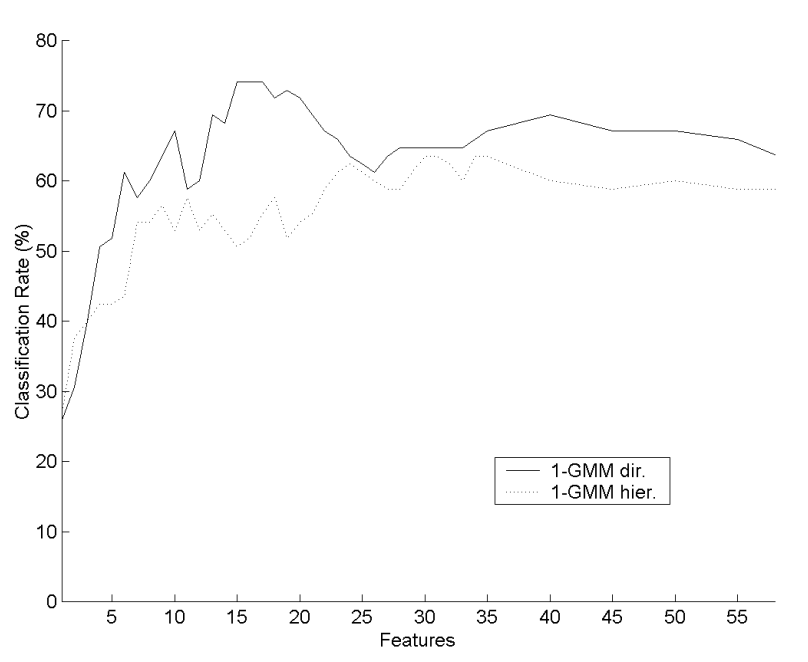
\includegraphics[scale=.2]{graph/curseofdimensionality}
			\end{figure}
		\end{frame}
		\begin{frame}{feature post-processing}{dimensionality reduction --- dimensionality issues 2/2}
            \begin{itemize}
                \item   \textbf{overfitting}:
                    \begin{itemize}
                        \item   lack of training data
                        \item   overly complex model
                        \item[$\Rightarrow$]<2-> model cannot be estimated properly
                    \end{itemize}
                    
                    \only<1-3>{
                    \figwithref{Overfitting}{\href{https://en.wikipedia.org/wiki/Overfitting}{https://en.wikipedia.org/wiki/Overfitting}}
                    %\begin{figure}
                        %\centering
                        %\includegraphics[scale=.3]{graph/overfitting}
                    %\end{figure}
                    }
                    \bigskip
                    \begin{itemize}
                        \item<3-> required training set size depends on 
                            \begin{itemize}
                                \item   classifier and its parametrization
                                \item   number of classes
                                \item   \ldots
                            \end{itemize}
                    \end{itemize}
                    \toremember{\textit{rule of thumb}:\\ don't bother if training set smaller than $\mathcal{F}^2$}
                \bigskip\item<5-> \textbf{curse of dimensionality}: increasing dimensionality leads to sparse training data
                    \begin{itemize}
                        \item   neighborhoods of data points become less concentrated
                        \item   model tends to be harder to estimate in higher-dimensional space
                    \end{itemize}
                %\pause
                %\item   \textbf{training set density}: 
                    %example: 1NN ($9$ training samples)
                    %\only<3>{
                        %$\mathcal{F} = 1$
                    %\begin{figure}
                        %\centering
                        %\includegraphics[scale=.3]{graph/1nn-1}
                    %\end{figure}
                    %}
                    %\only<4>{
                        %$\mathcal{F} = 2$
                     %\begin{figure}
                        %\centering
                        %\includegraphics[scale=.25]{graph/1nn-2}
                    %\end{figure}
                   %}
                    %\only<5>{
                        %$\mathcal{F} = 3$
                     %\begin{figure}
                        %\centering
                        %\includegraphics[scale=.25]{graph/1nn-3}
                    %\end{figure}
                   %}
                     %\vspace{50mm}
            \end{itemize}
		\end{frame}
		\begin{frame}{feature post-processing}{dimensionality reduction --- approaches}
			\begin{itemize}
				\item	\textbf{feature subset selection}:\\ discard least helpful features
                    \pause
                    \begin{itemize}
                        \item	high ``discriminative'' or descriptive power
                        \item	non-correlation to other features
                        \item	invariance to irrelevancies
                    \end{itemize}
				\bigskip
				\item<2->	\textbf{feature space transformation}:\\ map feature space
			\end{itemize}
		\end{frame}
		\begin{frame}{feature post-processing}{manual feature selection}
            \begin{columns}
            \column{.2\linewidth}
                example scatter plots of pairs of features in a multi-class scenario
            \column{.8\linewidth}
%                \begin{figure}
%                    \centering
%                    \hspace{-5mm}\vspace{-5mm}
                    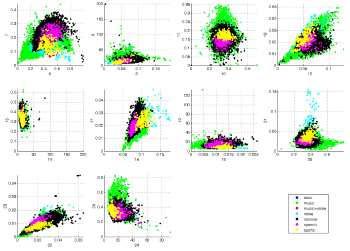
\includegraphics{noise_subfeatures}
%                \end{figure}
            \end{columns}
		\end{frame}
        
		\begin{frame}{feature post-processing}{feature subset selection: introduction}
			feature subset selection: 
			\begin{itemize}
				\item	\textbf{wrapper methods}:\\ use the ``classifier'' itself to evaluate feature performance
				\pause
				\item	\textbf{filter methods}:\\ use an objective function
			\end{itemize}
		\end{frame}

        \begin{frame}{excursion}{simple classifier~---~nearest neighbor}
            \begin{itemize}
                \item	    \textbf{training}: store the feature vector (with class label) of each training sample
                \item<2->	\textbf{classification}: for a new file/feature vector, detect the \textit{closest training vector} and choose its class as result
            \end{itemize}
            \vspace{-3mm}
            \only<1>{
                \figwithmatlab{Scatter}
            }
            \only<2->{
                \figwithref{Scatter-nn}{matlab source: matlab/displayScatter.m}
            }
        \end{frame}
        
		\begin{frame}{feature post-processing}{feature subset selection: wrapper methods 1/2}
			\begin{itemize}
				\item	\textbf{single variable classification}: evaluate each feature individually, choose the top $N$:\\
					subsets to test: $\mathcal{F}$
					
					\pause
					potential problems
					\begin{itemize}
						\item	inter-feature correlation is not considered
						\item	feature combinations are not considered
					\end{itemize}
				\pause
				\item	\textbf{brute force subset selection}: evaluate all possible feature combinations, choose the optimal:\\
					subsets to test: $2^\mathcal{F}$
			\end{itemize}
		\end{frame}
		\begin{frame}{feature post-processing}{feature subset selection: wrapper methods 2/2}
			\begin{itemize}
				\item	\textbf{sequential forward selection}: increase number of features step by step with the most promising feature
					
					\pause
					\begin{enumerate}
						\item	init: empty feature subset $\mathcal{V}_\mathrm{s} = {\emptyset}$
						\pause
						\item	find feature $v_j$ maximizing objective function
									\begin{equation}
										v_j = \argmax_{\forall j | v_j \notin \mathcal{V}_\mathrm{s}} J({\mathcal{V}_\mathrm{s}} \bigcup v_j) 
									\end{equation}
						\pause						
						\item	add feature $v_j$ to $\mathcal{V}_\mathrm{s}$ 
						\pause						
						\item	go to step $2$
					\end{enumerate}
				\pause
				\item	\textbf{sequential backward elimination}: decrease number of features step by step by discarding the least promising feature
				
				\pause
					\begin{enumerate}
						\item	init: full feature set
						\pause
						\item	find feature $v_j$ with the least impact on objective function
						\pause
						\item	discard feature $v_j$
						\pause
						\item	go to step $2$
					\end{enumerate}
			\end{itemize}
		\end{frame}
		\begin{frame}{feature post-processing}{feature subset selection: filter methods (PCA 1/2)}
			principal component analysis: map features to new coordinate system 
			\begin{equation}\label{eq:pca_an}
				\vec{u}(n) = \mat{T}^\mathrm{T}\cdot\vec{v}(n) 
			\end{equation}

			\pause
			transformation matrix ($\mathcal{F}\times\mathcal{F}$)	
			\begin{equation}
				\mat{T} =   \left[ 
					  			\begin{array}{cccc}
								\vec{c}_0 & \vec{c}_1 & \ldots & \vec{c}_{\mathcal{F}-1}\\
								\end{array}  
							\right] 
			\end{equation}

			\pause
			properties
			\begin{itemize}
			\item	$\vec{c}_i$ point in the direction of  highest \emph{variance}
			\pause
			\item	variance concentrated in as few output components as possible
			\pause
			\item	$\vec{c}_i$ orthogonal
					\begin{equation}
						\vec{c}_i^\mathrm{T}\cdot \vec{c}_j = 0\quad \forall\enspace i \neq j
					\end{equation}
			\item	transformation is invertible
					\begin{equation}\label{eq:pca_syn}
						\vec{v}(n) = \mat{T}\cdot\vec{u}(n)
					\end{equation}
			\end{itemize}
		\end{frame}
		\begin{frame}{feature post-processing}{feature subset selection: filter methods (PCA 2/2)}
			\figwithmatlab{Pca}
			
			\vspace{-5mm}
			\pause
			calculation of the transformation matrix
			\begin{enumerate}
				\item	compute covariance matrix $\mat{R}$
					\begin{equation}
						\mat{R} = \frac{1}{\mathcal{F}-1}\cdot \left(\vec{v} - \vec{\mu}_v\right)\left(\vec{v}^\mathrm{T} - \vec{\mu}^\mathrm{T}_v\right)
					\end{equation}
				\item	choose eigenvectors as axes for the new coordinate system
			\end{enumerate}
		\end{frame}

		\begin{frame}{feature post-processing}{PCA example}
            \only<1>{
                \textbf{pca input}
                \figwithref{PcaExample_input}{matlab source: matlab/displayPcaExample.m}
            }
            \only<2>{
                \textbf{pca output}
                \figwithref{PcaExample_output}{matlab source: matlab/displayPcaExample.m}
            }
             \only<3>{
            \textbf{pca eigenvalues}
                \figwithref{PcaExample_latent}{matlab source: matlab/displayPcaExample.m}
            }
            \only<4>{
            \textbf{pca transformation matrix}
                    \begin{equation}\left[ 
				  			\begin{array}{cccccc} 
   -0.4187 &   0.3467  & -0.4569  &  0.4143 &  -0.1271 &  -0.5549\\
   -0.3908 &   0.1815  &  0.8136  & -0.0289 &   0.2060 &  -0.3304\\
   -0.4516 &   0.3384  &  0.0859  &  0.2413 &  -0.2919 &   0.7285\\
   -0.4337 &   0.1699  & -0.3337  & -0.7243 &   0.3747 &   0.0816\\
    0.3802 &   0.5599  & -0.0381  &  0.2808 &   0.6622 &   0.1524\\
    0.3679 &   0.6245  &  0.0956  & -0.4071 &  -0.5267 &  -0.1495\nonumber
                             \end{array}  
		        	\right]         \end{equation}   }
            \only<5>{
            \textbf{pca transformation matrix}
                    \begin{equation}\left[ 
				  			\begin{array}{cccccc} 
   \textcolor{gtgold}{-0.4187} &   0.3467  & \textcolor{gtgold}{-0.4569}  &  0.4143 &  -0.1271 &  \textcolor{gtgold}{-0.5549}\\
   -0.3908 &   0.1815  &  \textcolor{gtgold}{0.8136}  & -0.0289 &   0.2060 &  -0.3304\\
   \textcolor{gtgold}{-0.4516} &   0.3384  &  0.0859  &  0.2413 &  -0.2919 &   \textcolor{gtgold}{0.7285}\\
   \textcolor{gtgold}{-0.4337} &   0.1699  & -0.3337  & \textcolor{gtgold}{-0.7243} &   0.3747 &   0.0816\\
    0.3802 &   \textcolor{gtgold}{0.5599}  & -0.0381  &  0.2808 &   \textcolor{gtgold}{0.6622} &   0.1524\\
    0.3679 &   \textcolor{gtgold}{0.6245}  &  0.0956  & -0.4071 &  \textcolor{gtgold}{-0.5267} &  -0.1495\nonumber
                             \end{array}  
		        	\right]         \end{equation}   }
            
		\end{frame}
	
    \section[summary]{lecture summary}
        \begin{frame}{summary}{lecture content}
            \begin{enumerate}
                \item   name examples for typical ways of computing derived features      
                \smallskip
                \item<2->   why is more features not always better
                \smallskip
                \item<3->   what is the difference between feature selection and feature mapping
                \smallskip
                \item<4->   describe two ways of selecting features
                \smallskip
                \item<5->   what does PCA and what are the advantages
            \end{enumerate}
        \end{frame}
\end{document}

